\documentclass{standalone}
\usepackage{tikz}
\usetikzlibrary{patterns, positioning}

\begin{document}
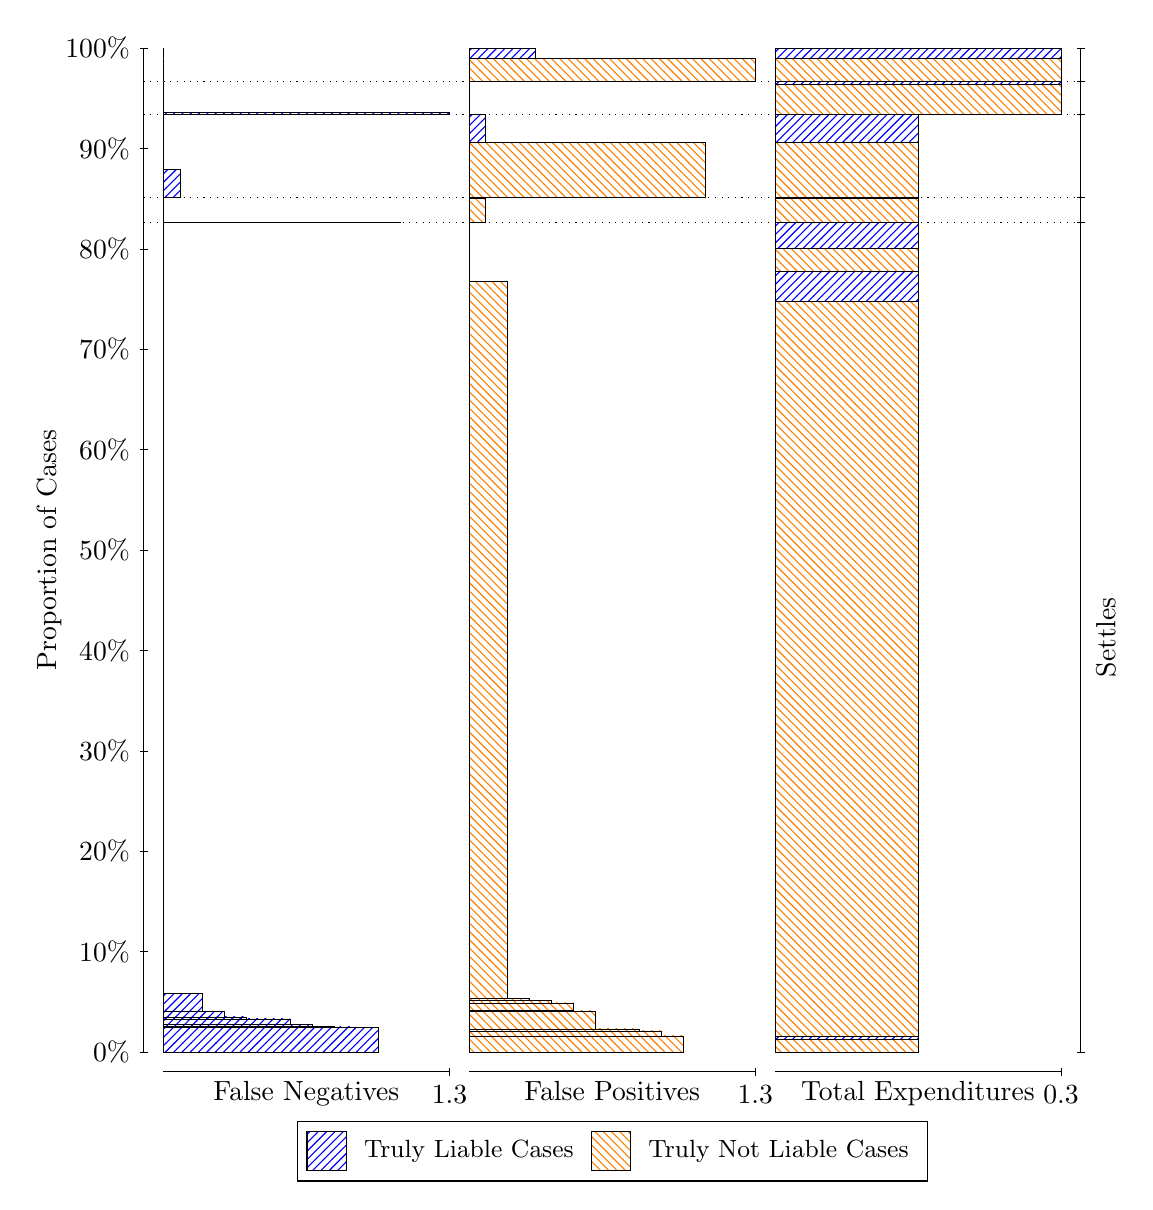
\begin{tikzpicture}
\draw[black, very thin] (1.5,1.75) -- (1.5,14.5);
\node[rotate=90, anchor=center] at (0.3, 8.125) {Proportion of Cases};
\draw[black, very thin] (1.45,1.75) -- (1.55,1.75);
\node[anchor=east] at (1.45, 1.75) {0\%};
\draw[black, very thin] (1.45,3.025) -- (1.55,3.025);
\node[anchor=east] at (1.45, 3.025) {10\%};
\draw[black, very thin] (1.45,4.3) -- (1.55,4.3);
\node[anchor=east] at (1.45, 4.3) {20\%};
\draw[black, very thin] (1.45,5.575) -- (1.55,5.575);
\node[anchor=east] at (1.45, 5.575) {30\%};
\draw[black, very thin] (1.45,6.85) -- (1.55,6.85);
\node[anchor=east] at (1.45, 6.85) {40\%};
\draw[black, very thin] (1.45,8.125) -- (1.55,8.125);
\node[anchor=east] at (1.45, 8.125) {50\%};
\draw[black, very thin] (1.45,9.4) -- (1.55,9.4);
\node[anchor=east] at (1.45, 9.4) {60\%};
\draw[black, very thin] (1.45,10.675) -- (1.55,10.675);
\node[anchor=east] at (1.45, 10.675) {70\%};
\draw[black, very thin] (1.45,11.95) -- (1.55,11.95);
\node[anchor=east] at (1.45, 11.95) {80\%};
\draw[black, very thin] (1.45,13.225) -- (1.55,13.225);
\node[anchor=east] at (1.45, 13.225) {90\%};
\draw[black, very thin] (1.45,14.5) -- (1.55,14.5);
\node[anchor=east] at (1.45, 14.5) {100\%};

\draw[black, very thin] (13.4,1.75) -- (13.4,14.5);
\draw[black, very thin] (13.35,1.75) -- (13.45,1.75);
\node[anchor=west] at (13.35, 1.75) {};
\draw[black, very thin] (13.35,12.286) -- (13.45,12.286);
\node[anchor=west] at (13.35, 12.286) {};
\draw[black, very thin] (13.35,12.602) -- (13.45,12.602);
\node[anchor=west] at (13.35, 12.602) {};
\draw[black, very thin] (13.35,13.655) -- (13.45,13.655);
\node[anchor=west] at (13.35, 13.655) {};
\draw[black, very thin] (13.35,14.073) -- (13.45,14.073);
\node[anchor=west] at (13.35, 14.073) {};
\draw[black, very thin] (13.35,14.5) -- (13.45,14.5);
\node[anchor=west] at (13.35, 14.5) {};

\draw[black, very thin, pattern color=blue, pattern=north east lines] (1.75,1.75) rectangle (4.475,2.0637);
\draw[black, very thin, pattern color=blue, pattern=north east lines] (1.75,2.0637) rectangle (4.1955,2.0695);
\draw[black, very thin, pattern color=blue, pattern=north east lines] (1.75,2.0695) rectangle (3.916,2.0755);
\draw[black, very thin, pattern color=blue, pattern=north east lines] (1.75,2.0755) rectangle (3.6365,2.1015);
\draw[black, very thin, pattern color=blue, pattern=north east lines] (1.75,2.1015) rectangle (3.3571,2.1705);
\draw[black, very thin, pattern color=blue, pattern=north east lines] (1.75,2.1705) rectangle (3.0776,2.1707);
\draw[black, very thin, pattern color=blue, pattern=north east lines] (1.75,2.1707) rectangle (2.7981,2.1959);
\draw[black, very thin, pattern color=blue, pattern=north east lines] (1.75,2.1959) rectangle (2.5186,2.2674);
\draw[black, very thin, pattern color=blue, pattern=north east lines] (1.75,2.2674) rectangle (2.2391,2.499);
\draw[black, very thin, pattern color=orange, pattern=north west lines] (1.75,2.499) rectangle (1.75,12.286);
\draw[black, very thin, pattern color=blue, pattern=north east lines] (1.75,12.286) rectangle (4.7545,12.29);
\draw[black, very thin, pattern color=orange, pattern=north west lines] (1.75,12.29) rectangle (1.75,12.602);
\draw[black, very thin, pattern color=blue, pattern=north east lines] (1.75,12.602) rectangle (1.9596,12.956);
\draw[black, very thin, pattern color=orange, pattern=north west lines] (1.75,12.956) rectangle (1.75,13.655);
\draw[black, very thin, pattern color=blue, pattern=north east lines] (1.75,13.655) rectangle (5.3833,13.687);
\draw[black, very thin, pattern color=orange, pattern=north west lines] (1.75,13.687) rectangle (1.75,14.073);
\draw[black, very thin, pattern color=orange, pattern=north west lines] (1.75,14.073) rectangle (1.75,14.364);
\draw[black, very thin, pattern color=blue, pattern=north east lines] (1.75,14.364) rectangle (1.75,14.5);
\draw[black, very thin, pattern color=orange, pattern=north west lines] (5.6333,1.75) rectangle (8.3583,1.9545);
\draw[black, very thin, pattern color=orange, pattern=north west lines] (5.6333,1.9545) rectangle (8.0788,2.0175);
\draw[black, very thin, pattern color=orange, pattern=north west lines] (5.6333,2.0175) rectangle (7.7994,2.0421);
\draw[black, very thin, pattern color=orange, pattern=north west lines] (5.6333,2.0421) rectangle (7.5199,2.0432);
\draw[black, very thin, pattern color=orange, pattern=north west lines] (5.6333,2.0432) rectangle (7.2404,2.2732);
\draw[black, very thin, pattern color=orange, pattern=north west lines] (5.6333,2.2732) rectangle (6.9609,2.2733);
\draw[black, very thin, pattern color=orange, pattern=north west lines] (5.6333,2.2733) rectangle (6.9609,2.3728);
\draw[black, very thin, pattern color=orange, pattern=north west lines] (5.6333,2.3728) rectangle (6.6814,2.4047);
\draw[black, very thin, pattern color=orange, pattern=north west lines] (5.6333,2.4047) rectangle (6.4019,2.4354);
\draw[black, very thin, pattern color=orange, pattern=north west lines] (5.6333,2.4354) rectangle (6.1224,11.537);
\draw[black, very thin, pattern color=blue, pattern=north east lines] (5.6333,11.537) rectangle (5.6333,12.286);
\draw[black, very thin, pattern color=orange, pattern=north west lines] (5.6333,12.286) rectangle (5.8429,12.598);
\draw[black, very thin, pattern color=blue, pattern=north east lines] (5.6333,12.598) rectangle (5.6333,12.602);
\draw[black, very thin, pattern color=orange, pattern=north west lines] (5.6333,12.602) rectangle (8.6378,13.301);
\draw[black, very thin, pattern color=blue, pattern=north east lines] (5.6333,13.301) rectangle (5.8429,13.655);
\draw[black, very thin, pattern color=orange, pattern=north west lines] (5.6333,13.655) rectangle (5.6333,14.041);
\draw[black, very thin, pattern color=blue, pattern=north east lines] (5.6333,14.041) rectangle (5.6333,14.073);
\draw[black, very thin, pattern color=orange, pattern=north west lines] (5.6333,14.073) rectangle (9.2667,14.364);
\draw[black, very thin, pattern color=blue, pattern=north east lines] (5.6333,14.364) rectangle (6.4718,14.5);
\draw[black, very thin, pattern color=orange, pattern=north west lines] (9.5167,1.75) rectangle (11.333,1.9122);
\draw[black, very thin, pattern color=blue, pattern=north east lines] (9.5167,1.9122) rectangle (11.333,1.95);
\draw[black, very thin, pattern color=orange, pattern=north west lines] (9.5167,1.95) rectangle (11.333,11.281);
\draw[black, very thin, pattern color=blue, pattern=north east lines] (9.5167,11.281) rectangle (11.333,11.664);
\draw[black, very thin, pattern color=orange, pattern=north west lines] (9.5167,11.664) rectangle (11.333,11.957);
\draw[black, very thin, pattern color=blue, pattern=north east lines] (9.5167,11.957) rectangle (11.333,12.286);
\draw[black, very thin, pattern color=orange, pattern=north west lines] (9.5167,12.286) rectangle (11.333,12.598);
\draw[black, very thin, pattern color=blue, pattern=north east lines] (9.5167,12.598) rectangle (11.333,12.602);
\draw[black, very thin, pattern color=orange, pattern=north west lines] (9.5167,12.602) rectangle (11.333,13.301);
\draw[black, very thin, pattern color=blue, pattern=north east lines] (9.5167,13.301) rectangle (11.333,13.655);
\draw[black, very thin, pattern color=orange, pattern=north west lines] (9.5167,13.655) rectangle (13.15,14.041);
\draw[black, very thin, pattern color=blue, pattern=north east lines] (9.5167,14.041) rectangle (13.15,14.073);
\draw[black, very thin, pattern color=orange, pattern=north west lines] (9.5167,14.073) rectangle (13.15,14.364);
\draw[black, very thin, pattern color=blue, pattern=north east lines] (9.5167,14.364) rectangle (13.15,14.5);
\draw[black, dotted] (1.5,12.286) -- (13.4,12.286);
\draw[black, dotted] (1.5,12.602) -- (13.4,12.602);
\draw[black, dotted] (1.5,13.655) -- (13.4,13.655);
\draw[black, dotted] (1.5,14.073) -- (13.4,14.073);
\draw[black, very thin] (1.75,1.5) -- (5.3833,1.5);
\node[anchor=north] at (3.5667, 1.5) {False Negatives};
\draw[black, very thin] (5.3833,1.45) -- (5.3833,1.55);
\node[anchor=north] at (5.3833, 1.45) {1.3};

\draw[black, very thin] (5.6333,1.5) -- (9.2667,1.5);
\node[anchor=north] at (7.45, 1.5) {False Positives};
\draw[black, very thin] (9.2667,1.45) -- (9.2667,1.55);
\node[anchor=north] at (9.2667, 1.45) {1.3};

\draw[black, very thin] (9.5167,1.5) -- (13.15,1.5);
\node[anchor=north] at (11.333, 1.5) {Total Expenditures};
\draw[black, very thin] (13.15,1.45) -- (13.15,1.55);
\node[anchor=north] at (13.15, 1.45) {0.3};

\node[black, centered, rotate=90] at (13.72, 7.0179) {Settles};





\draw (7.449999999999999,1.5) node[draw=none] (baseCoordinate) {};
\begin{scope}[align=center]
        \matrix[scale=0.5, draw=black, below=0.5cm of baseCoordinate, nodes={draw}, column sep=0.1cm]{
            \node[rectangle, draw, minimum width=0.5cm, minimum height=0.5cm, pattern=north east lines, pattern color=blue] {}; &
            \node[draw=none, font=\small] (B) {Truly Liable Cases}; &
            \node[rectangle, draw, minimum width=0.5cm, minimum height=0.5cm, pattern=north west lines, pattern color=orange] {}; &
            \node[draw=none, font=\small] (B) {Truly Not Liable Cases}; \\
            };
\end{scope}

\end{tikzpicture}
\end{document}